\section{Experimentación Y Resultados}

A continuación expondremos los resultados obtenidos por cada algoritmo para distintas imágenes. El objetivo será posteriormente hacer análisis de calidad subjetiva (es decir que vemos a simple vista), objetiva y tiempo de computos. Para, como dijimos en un principio, determinar ventajas y desventajas de cada uno de ellos. Para los análisis objetivos desarrollamos un programa en python que compara pixel a pixel basado en PSNR (Peak signal-to-noise ratio). Elegimos 3 casos particulares pero como se verá, los resultados son parecidos y se ha comportado de la misma manera en los otros ejemplos dados por la cátedra y lo mismo en otros ejemplos nuestros que no valían la pena ponerlos en el informe.

\subsection{Expermientación individual}

\subsubsection{Colores}


Se nos ocurrió que podría ser interesante chequear los comportamientos de estos procedimientos en una imagen con muchos bordes ya que estos, en algoritmos como el directional, son factores importantes y potencialmente conflictivos. Además hicimos que la imagen sea grande (5000 x 3000 pixeles) para poder analizar tiempos de computo y para influir en la calidad subjetiva, ya que si ponemos imágenes con mucha definición pequeños errores podrían pasar desapercividos para el ojo humano.

\begin{figure}

\begin{center}
       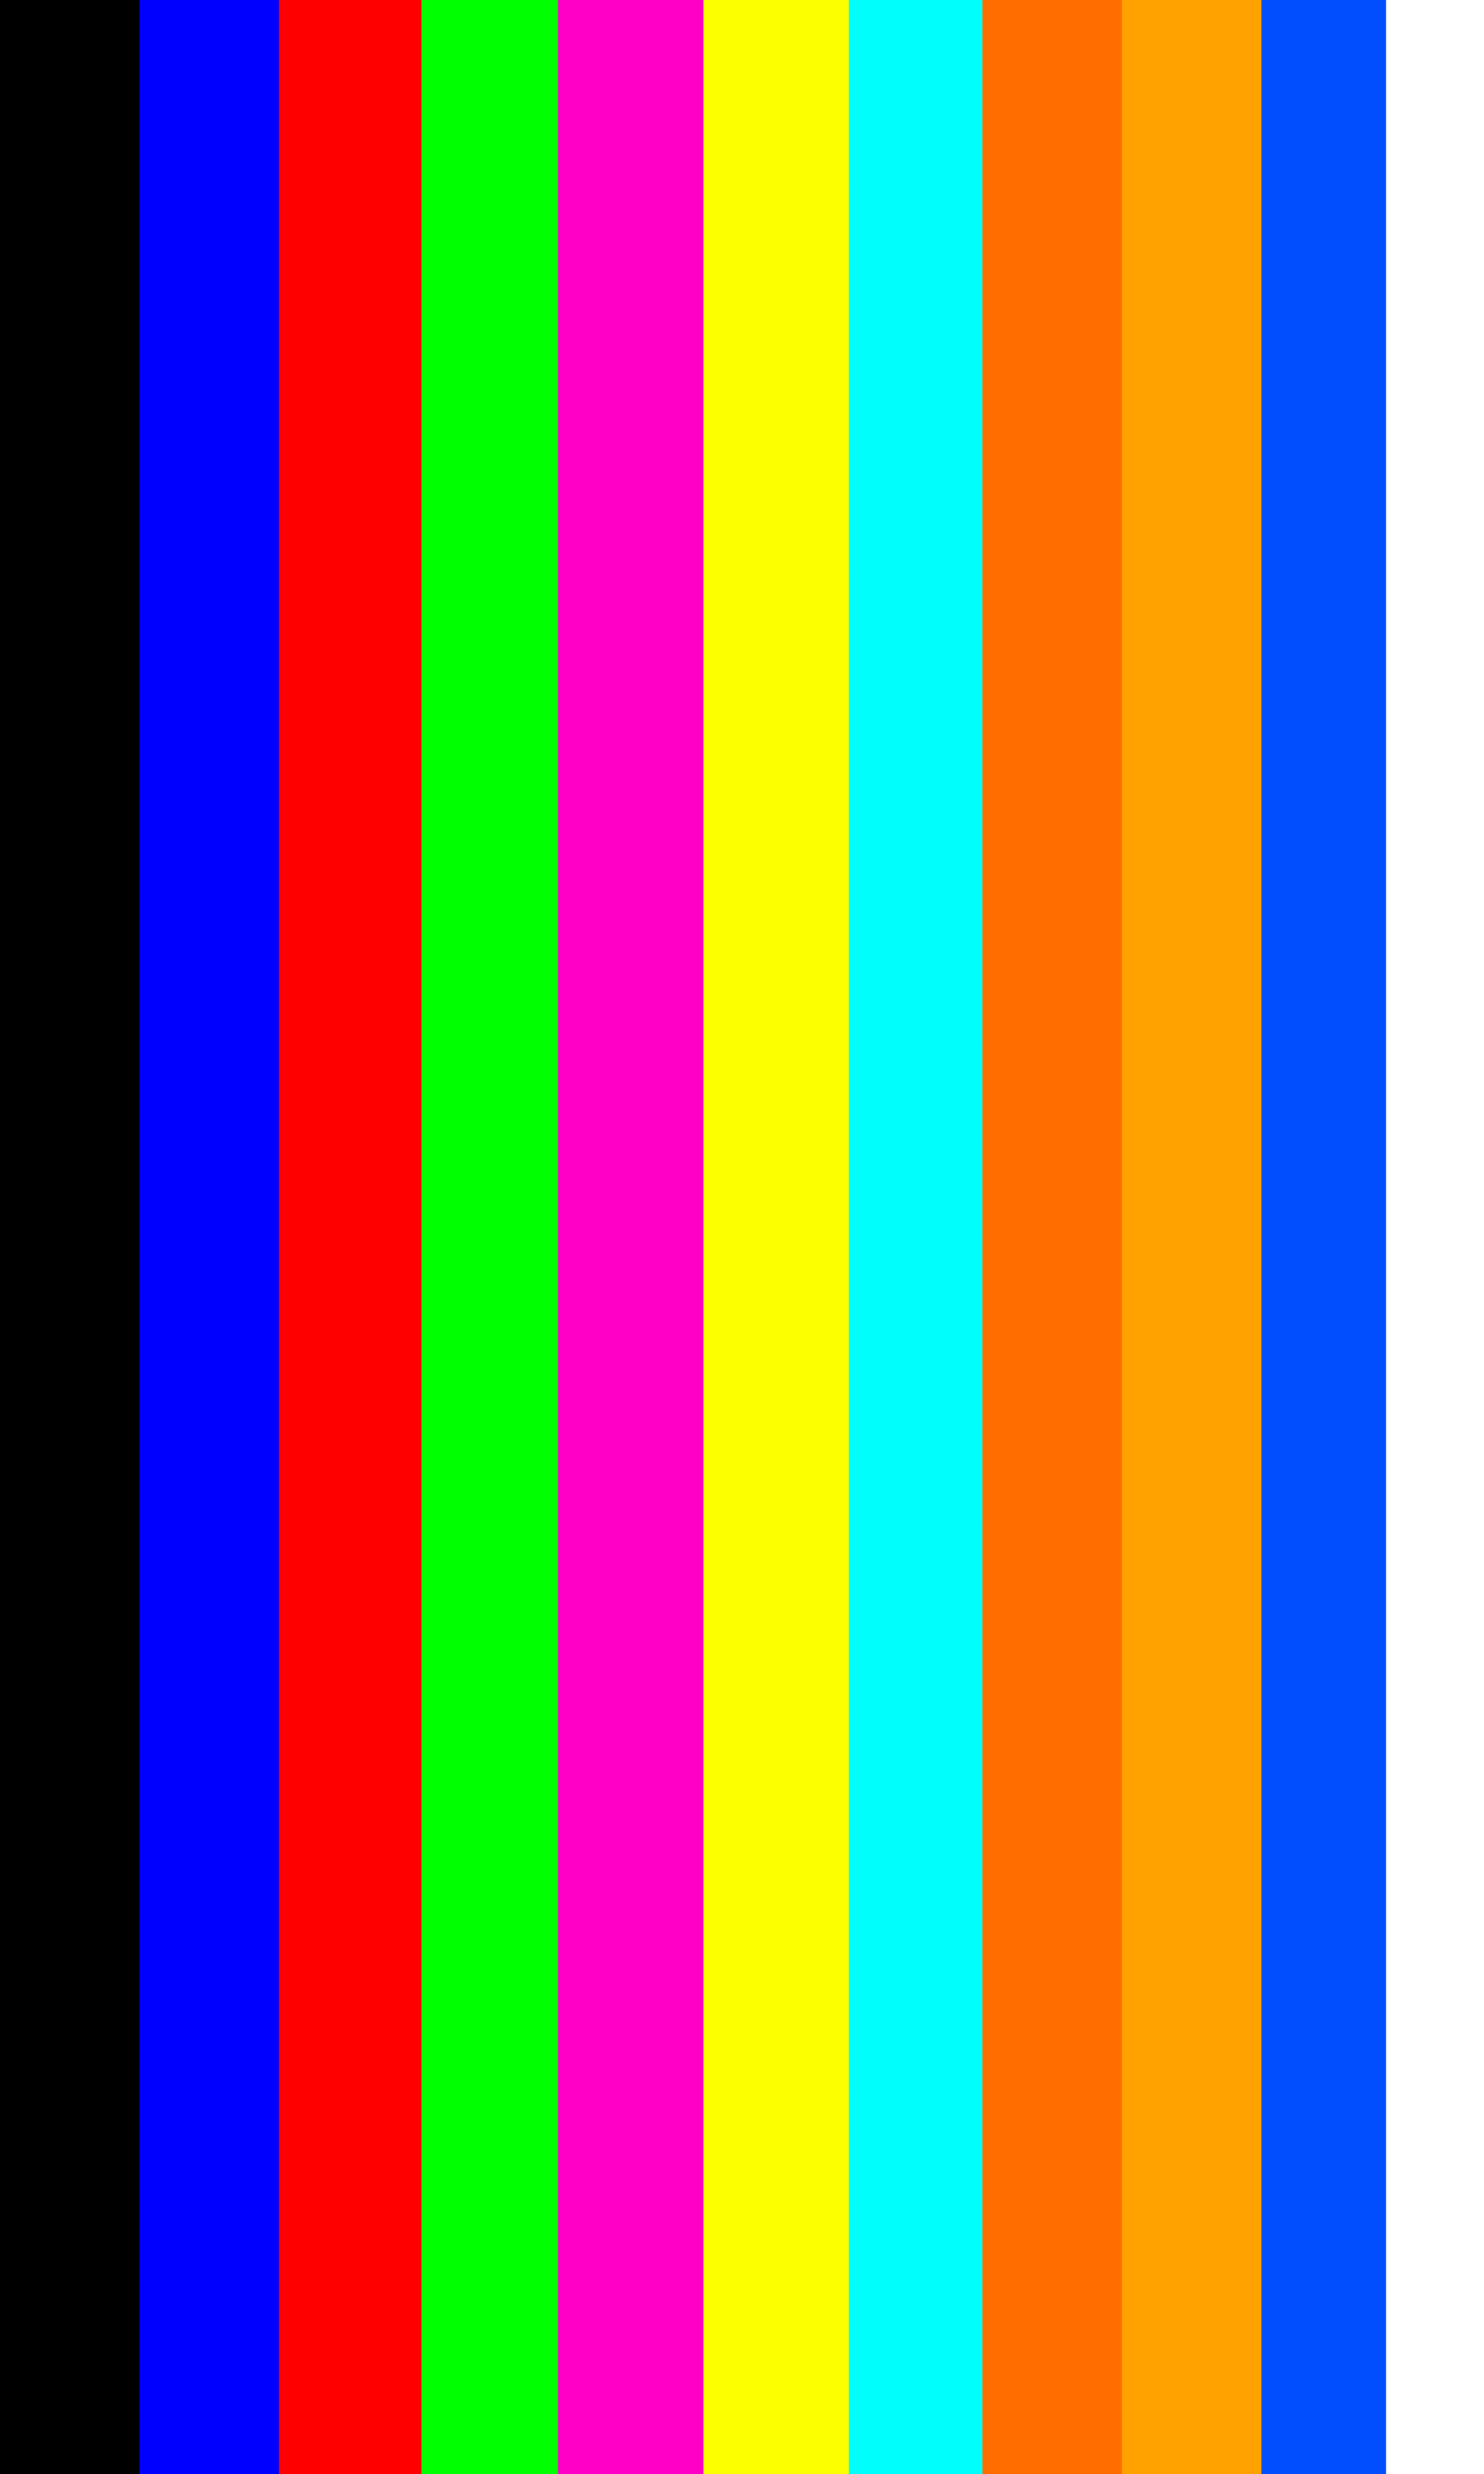
\includegraphics[scale=0.03]{imagenes/colores.png}
       \caption{Original }\label{fig:awesome_image1}
        \end{center}

\end{figure}

\newpage

Los resultados obtenidos a primera vista parecían todos iguales. Pero al hacerles zoom, pudimos ver que no era así. En la carpeta \textit{imagenes\_extra} que adejuntamos con el código se encuentran tanto la imagen original como sus respectivos resultados.
\begin{figure}[!htb]
\minipage{0.5\textwidth}
\begin{center}
    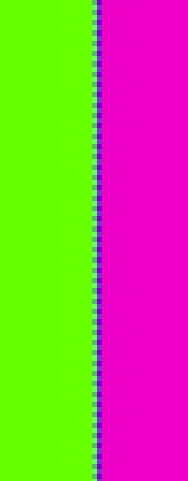
\includegraphics[scale=0.6]{imagenes/colores_bilineal_zoom.jpg}
    \caption{Bilineal Zoom}
        \end{center}
\endminipage
\minipage{0.5\textwidth}
\begin{center}
    
\includegraphics[scale=0.6]{imagenes/colores_hq_zoom.jpg}
    \caption{High Quality Zoom}
        \end{center}
\endminipage 
\end{figure}
\newpage
\begin{figure}[!htb]
\minipage{0.5\textwidth}
\begin{center}
    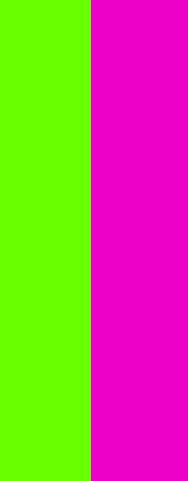
\includegraphics[scale=0.6]{imagenes/colores_directional_zoom.jpg}
    \caption{Directional Zoom}
        \end{center}
\endminipage
\minipage{0.5\textwidth}
\begin{center}
    
\includegraphics[scale=0.6]{imagenes/colores_vecinos_zoom.jpg}
    \caption{Vecinos Zoom}
        \end{center}
\endminipage 
\end{figure}


El algoritmo bilineal y el high quality tuvieron pequeños errores en los bordes. Podemos observar que en esos casos entre el verde y el violeta parece haber como una `cosedura' (\textit{zipper artifact}), la misma se repite en todos los bordes de la imagen. Estas diferencias imperceptibles por el tamaño de la imagen a primera vista pueden ser efectivamente comprobadas mediante un análisis de calidad objetivo. 

A continuación podemos ver los PSNR obtenidos al comparar los distintos resultados con la imagen original. Las im{ágenes que al hacerles zoom tenían esas $"$coseduras$"$ efectivamente fueron las que mas bajo PSNR dieron, es decir las que mas difirieron de la real.

$$ 
\begin{bmatrix}
           &      PSNR     \\
       highquality    &   39.67   \\
       bilineal       &   41.14   \\
       directional    &   48.13    \\
       vecinos        &   48.13      \\
\end{bmatrix} 
$$

A continuación veremos también cual fué el tiempo de computo de cada algoritmo.

$$ 
\begin{bmatrix}
           &      Tiempo (segundos)     \\
       directional    &   67.82    \\
       highquality    &   64.88   \\
       bilineal       &   63.00   \\
       vecinos        &   10.31      \\
\end{bmatrix} 
$$

Como era de esperarse, las proporciones de tiempo tienen sentido. Vecinos es el mas rápido ya que es el procedimiento mas simple y quality tarda mas que bilineal ya que antes aplica bilineal para luego mejorarlo (aunque en este caso no lo mejora). Para este caso tanto por calidad objetiva, subjetiva como en tiempo de cómputo vecinos parecería ser el mejor.


\clearpage
\subsubsection{Tablero de colores}
Dado que en la prueba anterior tuvimos un resultado muy fuerte (que el PSNR de vecinos dió mejor que el de HighQuality). Decidimos hacer otra prueba más con este mismo formato para poder investigar un poco más que pasó.
La imagen que tomamos fué la siguiente, que es parecida a la anterior en el sentido de que tiene muchos colores con límites bien drásticos,es decir que no hay cambios graduales de color sino que cambian de un pixel a otro. 
\begin{figure}[!htb]
\begin{center}
       
\includegraphics[scale=0.2]{imagenes/cuadrados_colores.png}
       \caption{Tablero de colores}
        \end{center}

\end{figure}

Podemos observar que además la imagen tiene una marca de agua. Decidimos utilizarla igual porque nos va a terminar siendo útil también en nuestras pruebas.Esta imagen también es mas chica ya que ahora no nos interesa tanto el tiempo de cómputo\\
Los resultados obtenidos tuvieron visibles diferencias a la imagen original. Las marcas de agua cambiaron de color (\textit{false color artifact}) en todos los casos y,a diferencia de la prueba anterior, el resultado de vecinos tuvo claros errores en los bordes mientras que los otros a simple vista parecería que no. No exponemos estos resultados para no sobre cargar de imágenes el informe pero dejamos adjunta la imagen original por si se desea corroborar esto haciendo uno mismo los tests.\\
\paragraph{Calidad cuantificable}
Yendo a la parte que más nos interesaba, la calidad cuantificable. Podemos observar que ahora si tuvo un comportamiento mas intuitivo.

$$ 
\begin{bmatrix}
           &      PSNR     \\
       highquality    &   38.58   \\
       bilineal       &   36.08  \\
       directional    &   34.90    \\
       vecinos        &   32.00      \\
\end{bmatrix} 
$$

Efectivamente la mejor esta vez fué el highquality y el peor vecinos. También tiene sentido que spline(direccional) haya sido peor en calidad ya que depende de toda la fila y columna mientras otros dependen de sus valores más próximos.
\paragraph{Tiempos}
A continuación veremos cual fué el tiempo que tomó cada algoritmo.

$$ 
\begin{bmatrix}
           &      Tiempo (segundos)     \\
       directional    &   4.46    \\
       highquality    &   4.21   \\
       bilineal       &   4.14   \\
       vecinos        &   0.15      \\
\end{bmatrix} 
$$

\clearpage
\subsubsection{Imagen 9 - Avión}

Nos pareció interesante hacer un análisis particular de la Imagen 9 ya que posee varias características en donde se pueden observar diferentes condiciones para ver como actúan los cuatro algoritmos, estos son: tener gran cantidad de sectores bordes, gran variedad de colores que contrastan altamente y principalmente tener texto. Destacamos esto último ya que una de las cualidades más importantes que deben poseer estos algoritmos es la de asegurar nitidez y suavidad, detalles que se ven al procesar imágenes que poseen texto. \\
A continuación mostraremos el resultado de los algoritmos para esta imagen:

\begin{figure}[h]
\begin{center}
       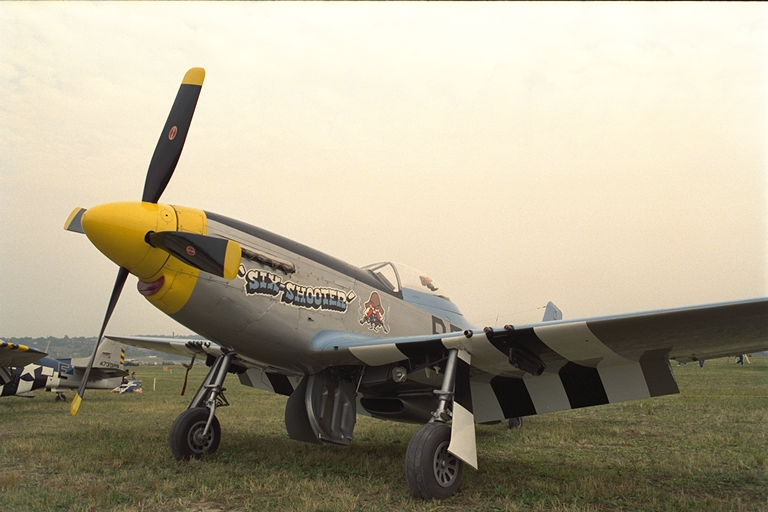
\includegraphics[width=0.5\textwidth]{imagenes/img9.png}
        \caption{Imagen original}
\end{center}
\end{figure}

\begin{figure}[h]
       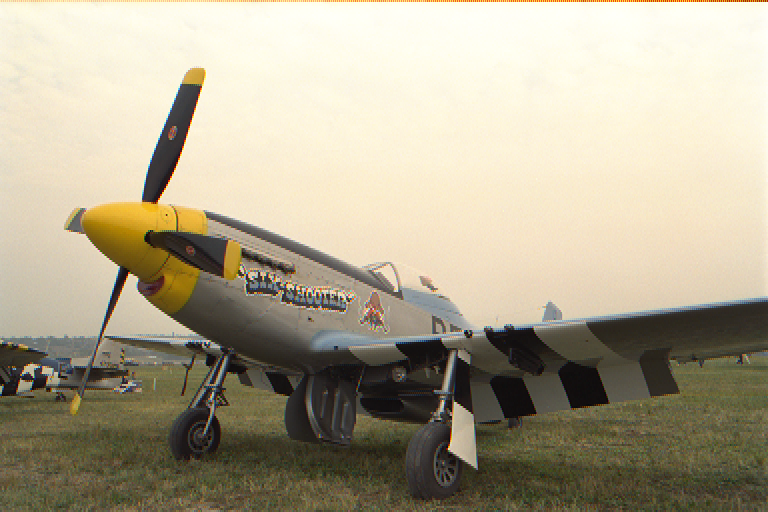
\includegraphics[width=0.5\textwidth]{imagenes/img9_demosicing_vecino.png}
           \hfill
        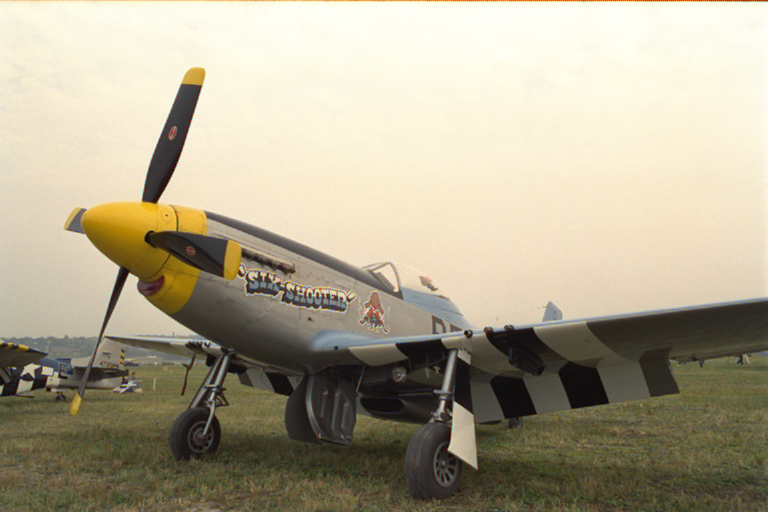
\includegraphics[width=0.5\textwidth]{imagenes/img9_demosicing_bilineal.png}
        Algoritmos de Vecinos e Interpolación Bilineal
\end{figure}


\begin{figure}[h]
       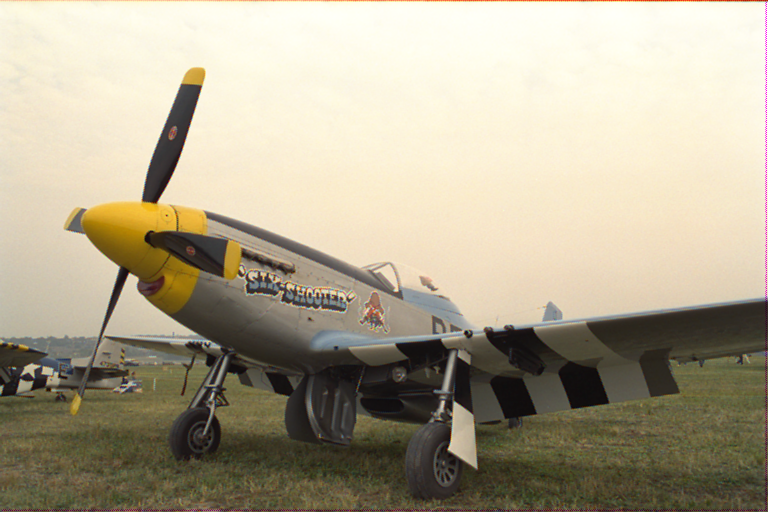
\includegraphics[width=0.5\textwidth]{imagenes/img9_demosicing_spline.png}
           \hfill
        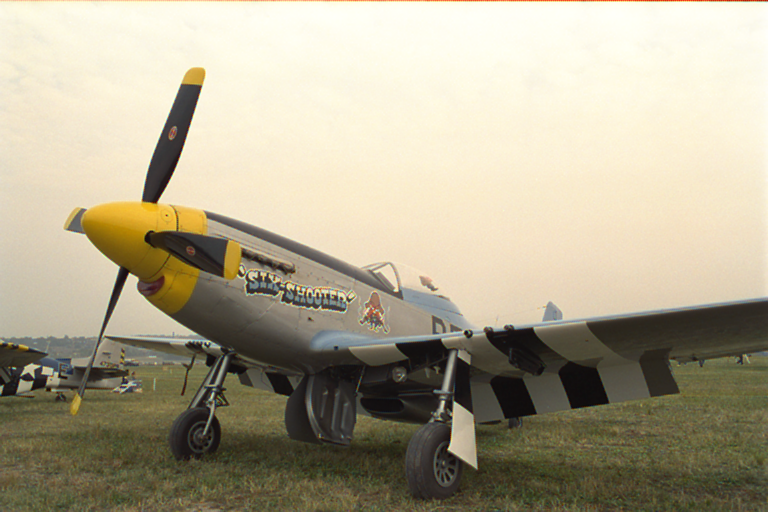
\includegraphics[width=0.5\textwidth]{imagenes/img9_demosicing_quality.png}
        Algoritmos de Interpolación Direccional y HighQuality
\end{figure}
\newpage

Como se puede observar, a simple vista pareciera que los 4 algoritmos dan un resultado bastante aceptable, pero mirando detalladamente y comparando entre sí se puede observar una gran diferencia entre ellos, principalmente en zonas borde y en la zona del texto del avión. Subjetivamente pareciera ser que la imagen más parecida a la original es la del HighQuality, seguida por la Interpolación Direccional, pero objetivamente en base a los resultados obtenidos al método PSNR se observa que el algoritmo de Interpolación Bilineal supera al Direccional, algo que llama bastante la atención y que indica que lo subjetivo se diferencia bastante de los objetivo. 

$$ 
\begin{bmatrix}
        algoritmo   &      PSNR     \\
       highquality    &   37.71  \\
       bilineal    &     35.34  \\
       directional    &      33.35    \\
       vecinos   &      30.49     \\
\end{bmatrix} 
$$
Yendo más a fondo aún en la cuestión y para mostrar el nivel de detalle que obtiene cada algoritmo, decidimos hacer zoom en la zona donde la imagen posee texto:

\begin{figure}
       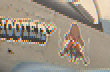
\includegraphics[width=0.5\textwidth]{imagenes/img9_demosicing_vecino_cropped.png}
        \caption{Vecinos}
\end{figure}

\begin{figure}
       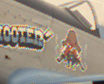
\includegraphics[width=0.5\textwidth]{imagenes/img9_demosicing_bilineal_cropped.png}
        \caption{Bilineal}
\end{figure}

\begin{figure}
       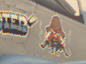
\includegraphics[width=0.5\textwidth]{imagenes/img9_demosicing_spline_cropped.png}
        \caption{Direccional}
\end{figure}

\begin{figure}
       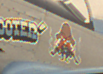
\includegraphics[width=0.5\textwidth]{imagenes/img9_demosicing_quality_cropped.png}
        \caption{Quality}
\end{figure}

Acá si se puede observar la nitidez y suavidad que presenta cada algoritmo, viéndose como mejora la calidad del texto para cada imagen y como va disminuyendo el ruido aumentando la refinación alrededor del mismo.

\newpage

\subsubsection{Imagen 12}

A continuación probaremos con una imagen provista por la cátedra para tener mas resultados sobre los cuales apoyarnos a la hora de sacar nuestras conclusiones. Obviaremos la imagen bayerizada ya que sólo
nos interesaba ver que sea correcta la bayerización y con lo ya hecho eso queda claro.

\begin{figure}[h]
\begin{center}
       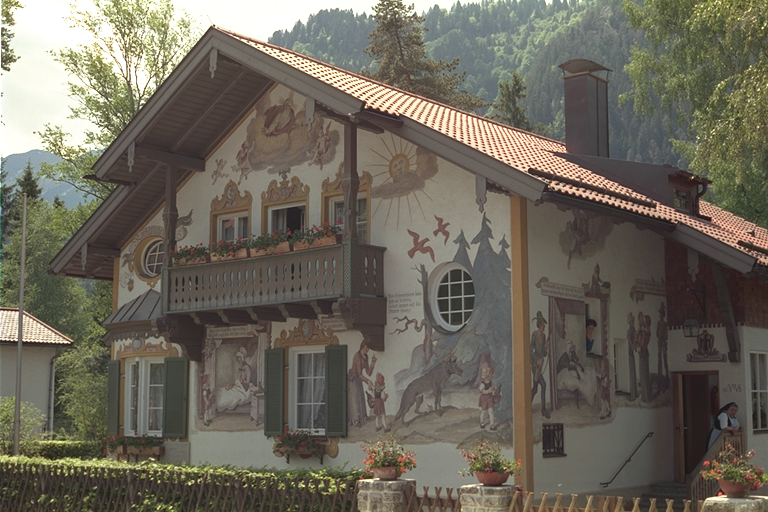
\includegraphics[scale=0.3]{imagenes/img12.png}
       \caption{Original }\label{fig:awesome_image1}
        \end{center}

\end{figure}

\begin{figure}[!ht]
\minipage{0.5\textwidth}
\begin{center}
    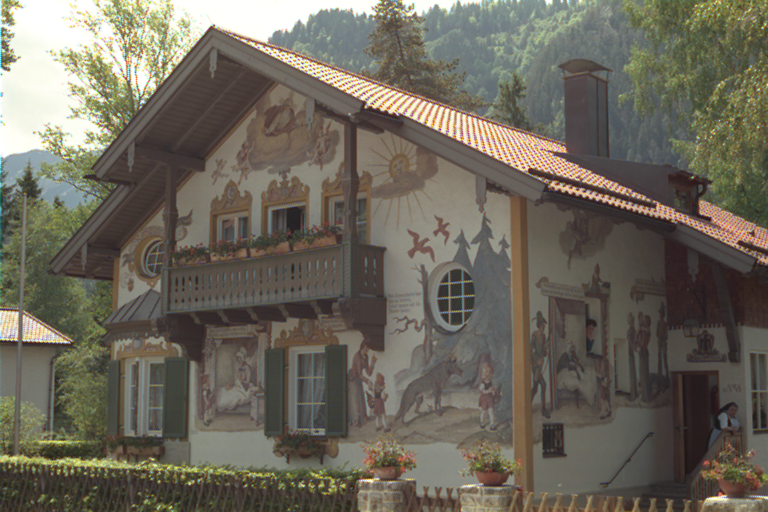
\includegraphics[scale=0.3]{imagenes/img12_demosicing_bilineal.png}
    \caption{Bilineal }
 \end{center}
\endminipage
\minipage{0.5\textwidth}
\begin{center}
    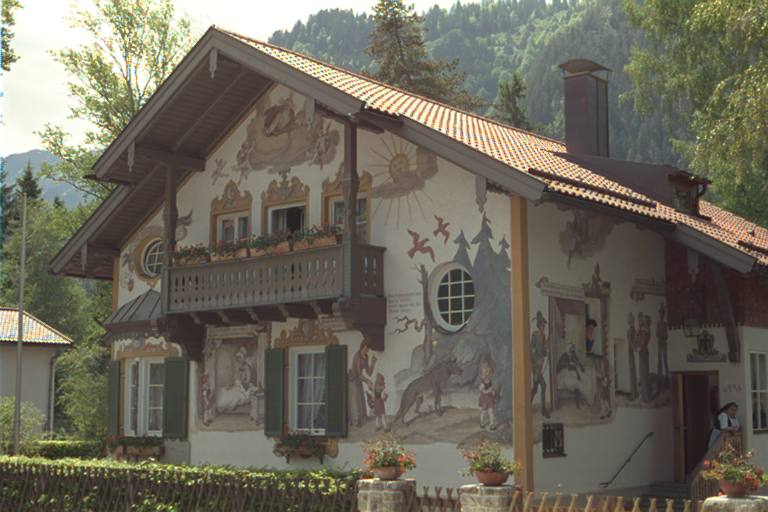
\includegraphics[scale=0.3]{imagenes/img12_demosicing_quality.png}
    \caption{High Quality}
        \end{center}
\endminipage\hfill
\end{figure}

\begin{figure}[h]
\minipage{0.5\textwidth}
\begin{center}
    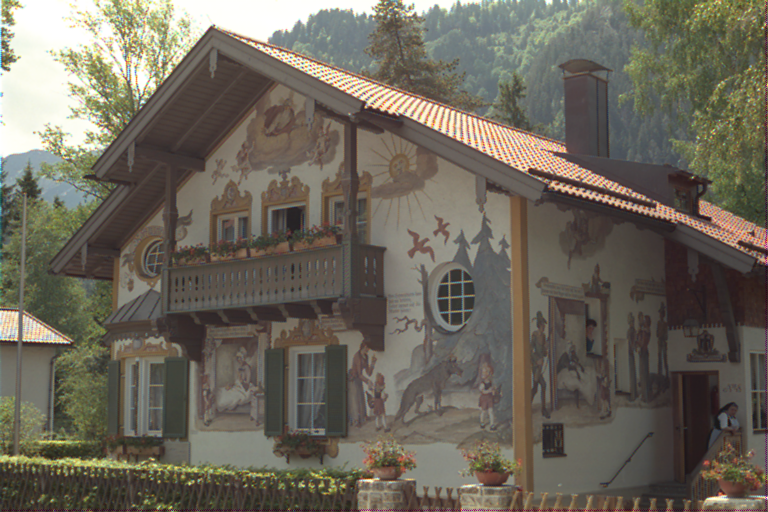
\includegraphics[scale=0.3]{imagenes/img12_demosicing_spline.png}
    \caption{Directional}
        \end{center}
\endminipage
\minipage{0.5\textwidth}
\begin{center}
    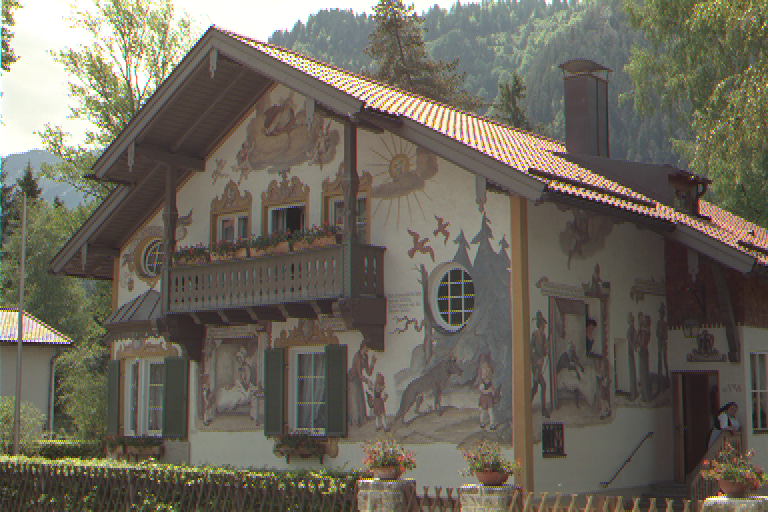
\includegraphics[scale=0.3]{imagenes/img12_demosicing_vecino.png}
    \caption{Vecinos}
 \end{center}
\endminipage
 
\end{figure}
\newpage

Subjetivamente highquality parece ser la mejor. Ya que se la ve bastante menos borrosa que las demás y con bordes mas nítidos, esto es facilmente apreciable en los dibujos que hay sobre la casa. A diferencia de vecinos que tiene bordes no sólo poco nítidos sino hasta claramente pixelados. Entre Directional y bilineal podemos notar que el primero, en los dibujos de la casa, es un poco más nitido que el segundo y parece tener un poco mas de calidad, también apreciable en los dibujos de la casa.

Veamos ahora a través del calculo del PSNR contra la imagen original como es el ranking.

$$ 
\begin{bmatrix}
           &      PSNR    \\
       quality    &   32.33   \\
       bilineal    &      30.27   \\
       directional    &      29.87    \\
       vecinos   &      25.45     \\
\end{bmatrix} 
$$

Objetivamente el peor y el mejor se mantienen, debido a que quality es el de mayor PSNR y vecinos el de menor. En estos valores también es apreciable la gran diferencia de resultados observada anteriormente, mientras que subjetivamente se podía notar una nítida y la otra directamente pixelada objetivamente el PSNR es 10 puntos mas grande en la quality. Lo que si cambia acá es la relación entre directional y bilineal, mientras que objetivamente el bilineal parecía ser mejor subjetivamente podemos ver que esto es al revés (aunque también por poca diferencia).

Como dato interesante vale aclarar que en el tejado de la casa podemos ver anomalías en todos los resultados, así como también en los arboles que están a la izquierda y por encima. Más adelante analizaremos bien porque es que sucede esto.

\subsection{Experimentación comparativa}

\newpage
\subsubsection{Comparación de tiempos}

En esta sección presentaremos una comparativa entre los tiempos que tarda cada algoritmo a medida que aumenta el tamaño de la imagen. Para tal fin testamos cada algoritmo con 2 tipos de imágenes cuadradas generadas que van aumentando su tamaño, una con pixeles de colores aleatorios y la otra con todos los pixeles del mismo color, es decir, plana. Creemos que es una forma correcta de comparar los tiempos ya que usamos la misma instancia para cada prueba y además utilizamos estas dos instancias para comprobar si la complejidad de los algoritmos se ve influenciada por la información que contiene la imagen además del tamaño.

A continuación el gráfico con la comparación de tiempos entre los 4 algoritmos para una imagen generada aleatoriamente:


\begin{figure}[h]
       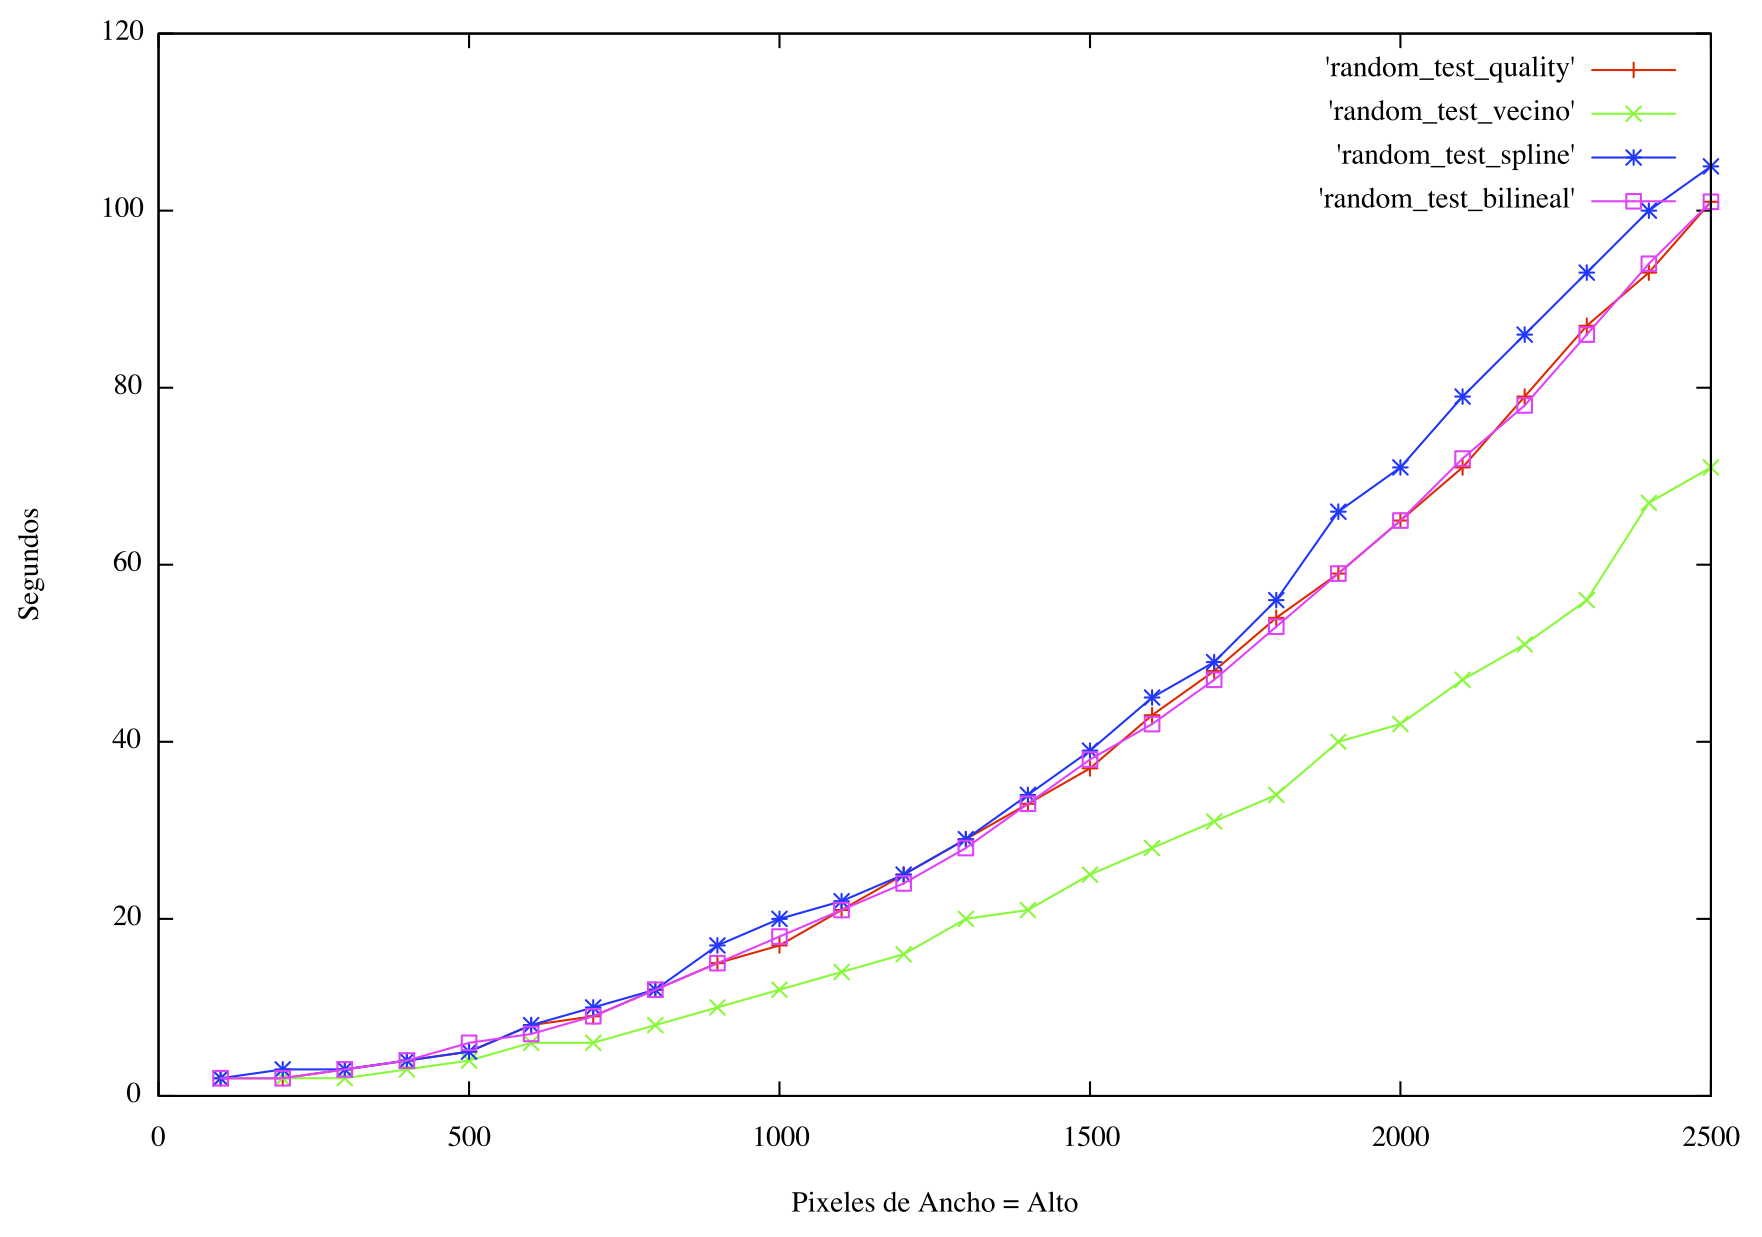
\includegraphics[width=1\textwidth]{imagenes/tiempo_algoritmos_random.png}
\end{figure}



\begin{figure}[h]
       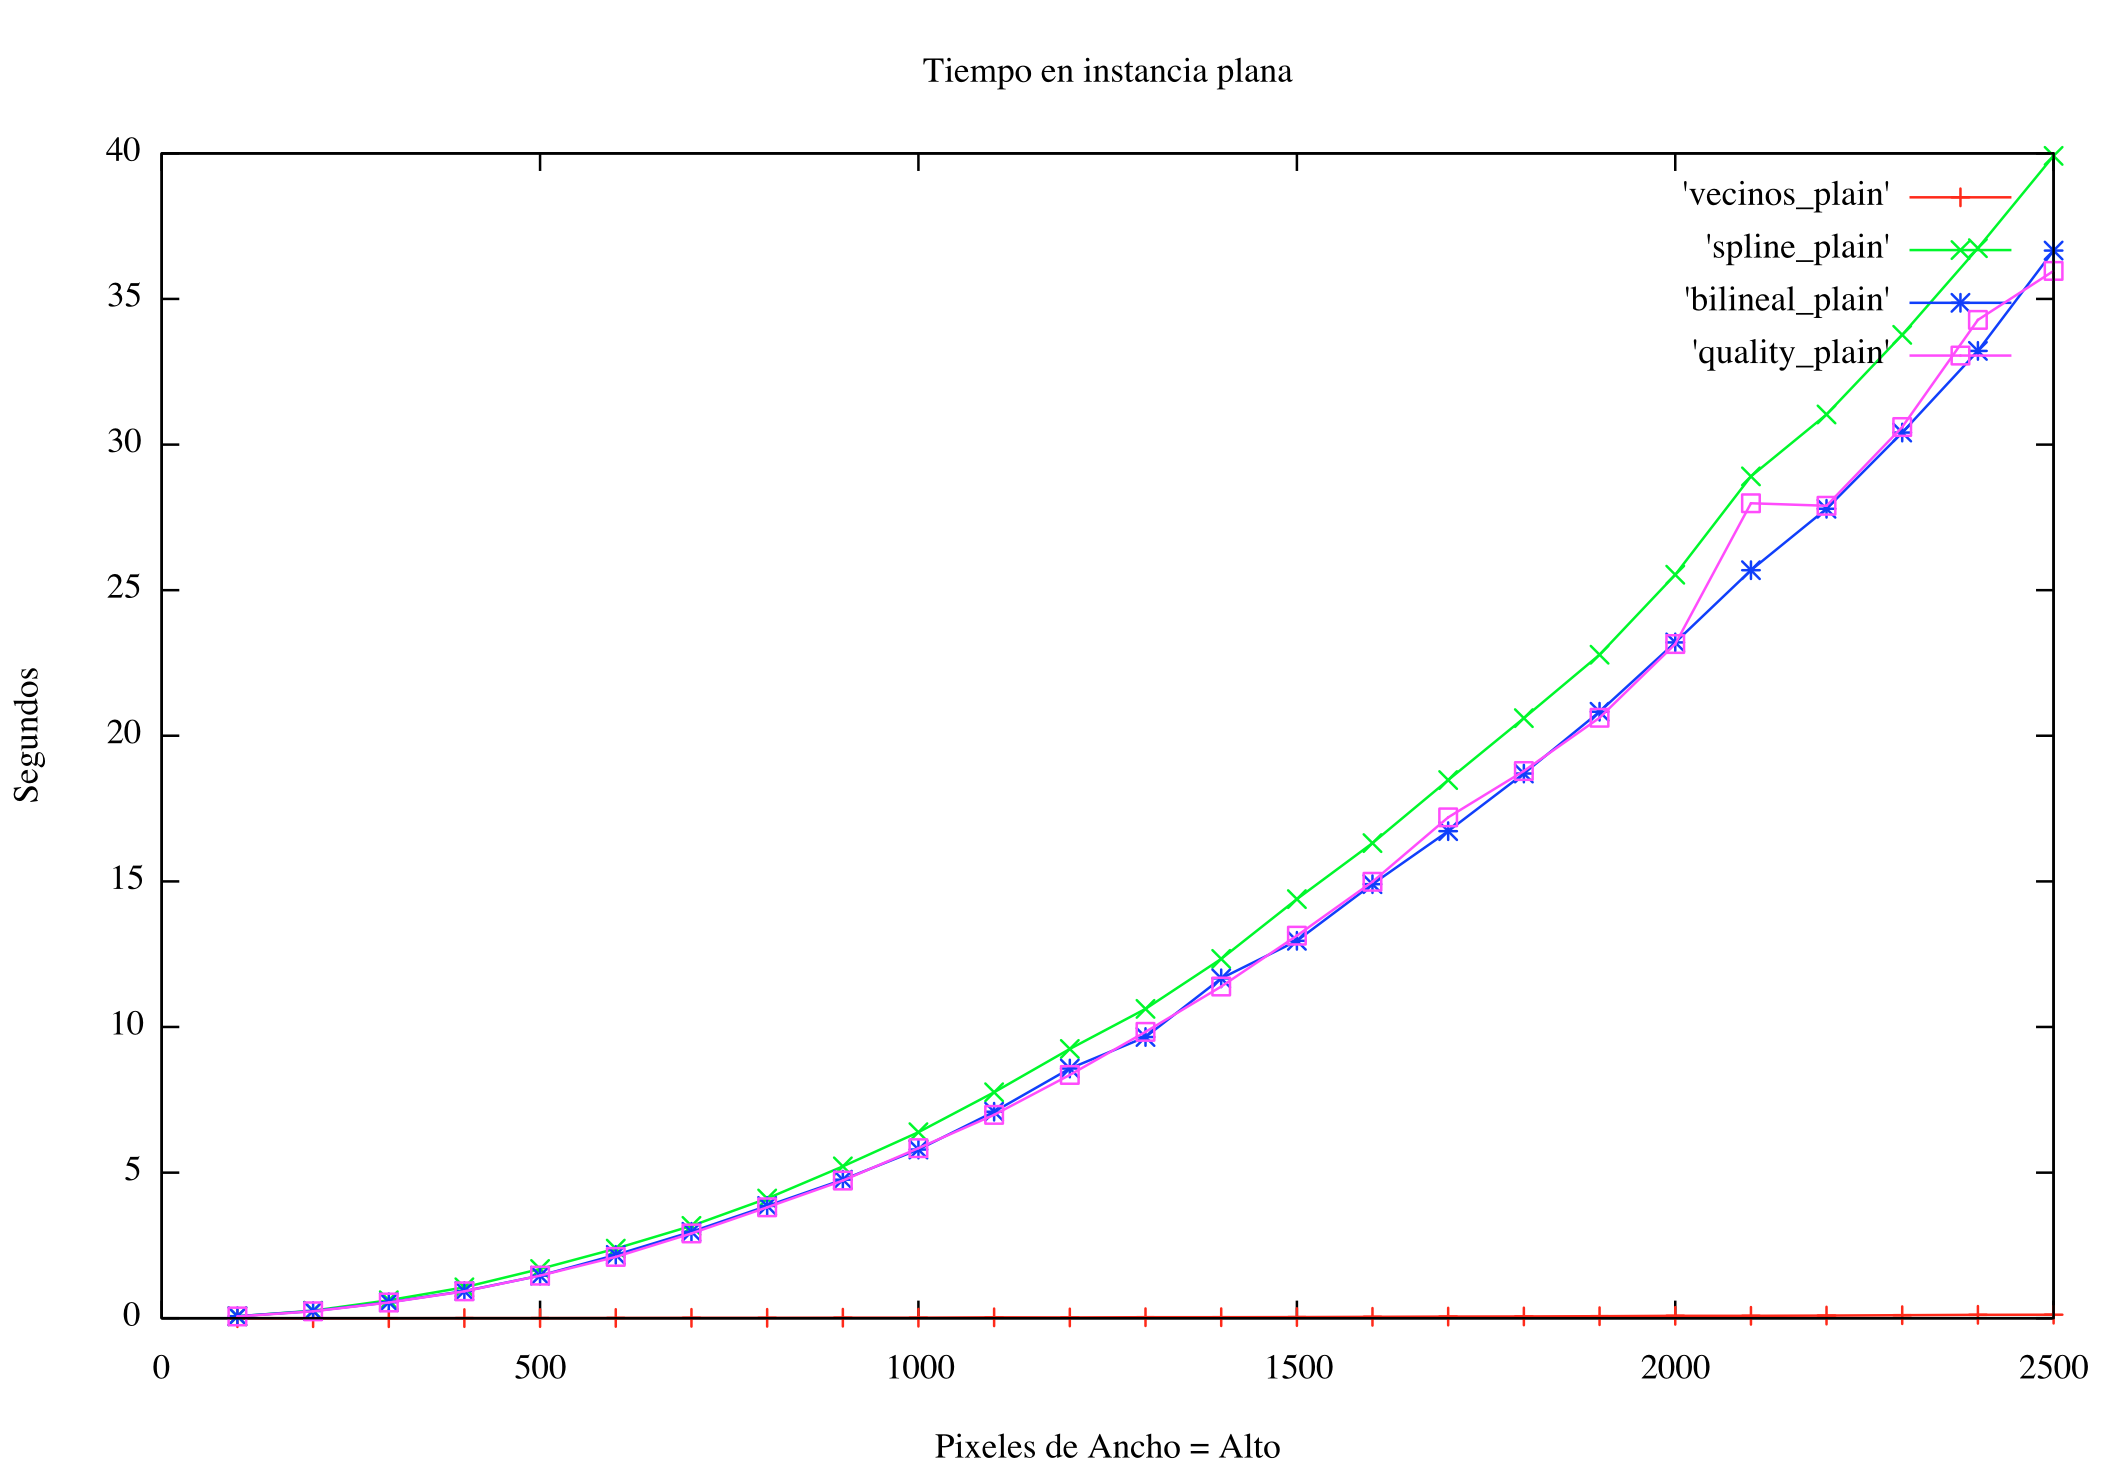
\includegraphics[width=1\textwidth]{imagenes/tiempo_algoritmos_plain.png}
\end{figure}



Vecinos al ser el más simple, tiene sentido que haya tardado menos. Lo único que hace es recorrer la imagen y rellenar por cada color faltante de cada pixel, de, valga la redundancia, sus vecinos que captaron ese color en la bayerización. Bilineal en segundo puesto, ya que realiza un promedio y necesita ver más puntos. \\
Tanto Direccional y Quality, utilizan bilineal ya que no son algoritmos de aproximación de cero, si no de mejora. Por lo que ya tienen una cota inferior. Igualmente es notable que Quality siendo el mejor resultado, como venimos viendo en puntos anteriores y un detalle mejor en la próxima sección, también sea el de menor tiempo. Esto se debe a que tiene una cuenta parecida al bilineal pero en pocos píxeles, a diferencia de Direccional que resuelve un sistema de ecuaciones por cada fila y columna.\\
Igualmente no es poco notar que son bastantes lentos los algoritmos, y las pruebas si bien fueron con imágenes relativamente grandes, no alcanzan a las cámaras promedio que claramente no tardan 10 segundos en resolver la foto final. O existen optimizaciones que no llegamos a hacer o hay un mejor aprovechamiento del hardware, paralelismo, etc.
Como el algoritmo de HighQuality solamente procesa los verdes de la imagen luego de primero utilizar el algoritmo Bilineal, el tiempo que tardará es el de este último más el tiempo del agregado para que las imágenes tengan una mayor calidad para el color verde.
Por último se puede observar que como creíamos, los tiempos que tardan los algoritmos comparando las dos instancias para cada tamaño es casi idéntico, por lo que podemos concluir que el contenido de la imagen a procesar no es tan influyente como si lo es el tamaño de la misma.  

\textit{Para los experimentos incluimos dos archivos random.sh y plain.sh para simular los mismos}


\subsubsection{Comparación de calidad}
En esta sección compararemos solo los verdes de las imágenes y veremos los resultados utilizando PSNR. Recordemos que este término, calcula nivel de ruido en una señal.

\begin{figure}[h]
       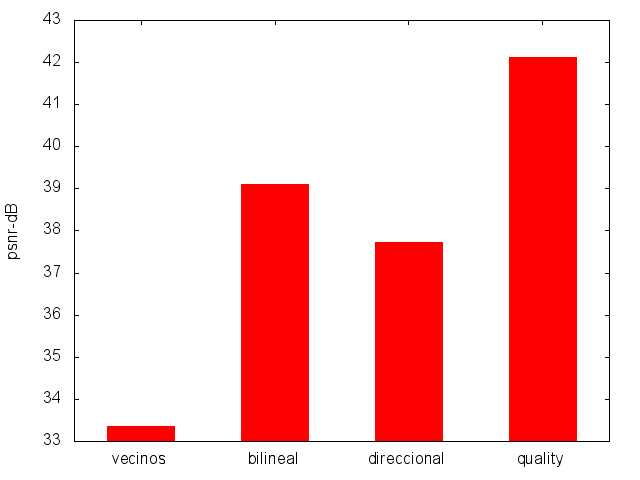
\includegraphics[scale=0.8]{imagenes/quality_performance.png}
       \caption{Img1}
\end{figure}

Como venimos viendo en otros ejemplos, img9 y este, como era esperado, el vecinos es el que peor hizo, y quality fue el mejor. Sin embargo notemos que Spline si bien 
tendría que tener un valor mayor que bilineal ya que subjetivamente notamos mejora entre ellos, no lo tiene, es 
decir, el nivel de ruido es mayor en el direccional. Esto tiene sentido en la medida que el algoritmo direccional 
utiliza toda la fila y toda la columna para calcular el valor de las coordenadas $b_j$, $c_j$ y $d_j$ por lo que está 
sujeto a valores distintos al valor final, a diferencia de Bilineal que está sujeto a sus vecinos directos que es 
mucho más probable que tengan un valor más próximo. 

\subsubsection{Calidad subjetiva}

En las secciones anteriores analizamos la calidad de las imágenes basándonos en los valores de los pixeles que resultaban después de aplicar los distintos algoritmos de demosaicing y la comparamos con la original pero no teníamos en cuenta las diferencias entre estas a la vista del ojo humano. Por esto último en esta sección mediremos la calidad subjetiva de las imágenes en base a los \textbf{artifacts} que se pueden encontrar en cada una de ellas.\\
Lo llamativo es que en mayor o menor intensidad los artifacts aparecen en los 4 algoritmos:

\paragraph{Moiré / False color}
Ocurre en los 4 algoritmos por igual
\begin{figure}[h]
\minipage{0.5\textwidth}
\begin{center}
       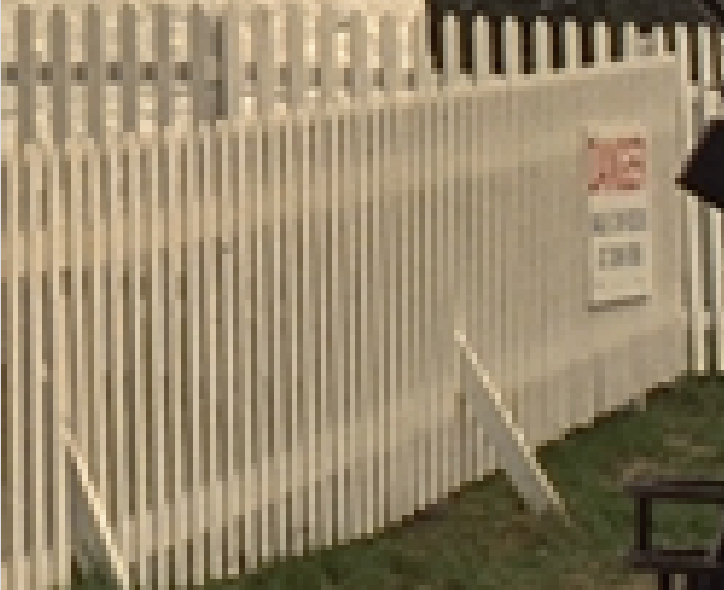
\includegraphics[width=0.5\textwidth]{imagenes/img8_moire_original.png}
        \caption{Original}
        \end{center}
\endminipage
\minipage{0.5\textwidth}
\begin{center}
       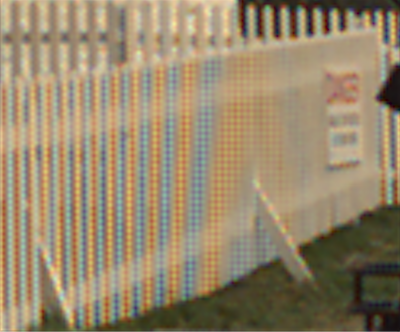
\includegraphics[width=0.5\textwidth]{imagenes/img8_moire.png}
        \caption{}
         \end{center}
\endminipage
\end{figure}
\paragraph{Zippering}

Si bien aparece en todos los algoritmos, en el de \textit{Vecinos} aparece en mayor intensidad y siendo muy notorio.

\begin{figure}[h]
\minipage{0.5\textwidth}
\begin{center}
       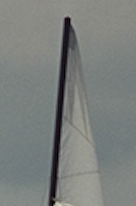
\includegraphics[width=0.5\textwidth]{imagenes/img5_zippering_original.png}
        \caption{Original}
        \end{center}
\endminipage
\minipage{0.5\textwidth}
\begin{center}
       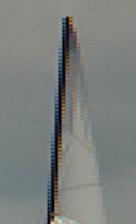
\includegraphics[width=0.5\textwidth]{imagenes/img5_zippering.png}
        \caption{}
         \end{center}
\endminipage
\end{figure}


\paragraph{Blur}

\begin{figure}[h]
\minipage{0.5\textwidth}
\begin{center}
       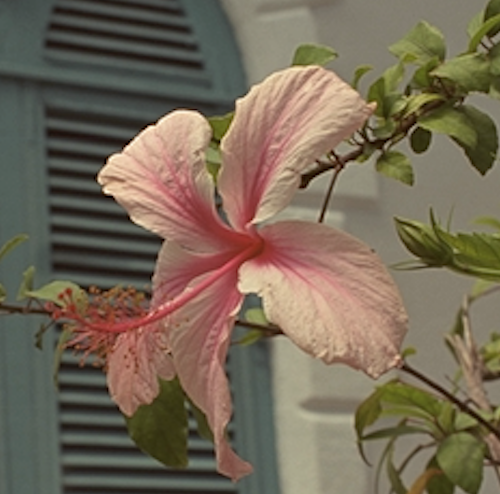
\includegraphics[width=0.5\textwidth]{imagenes/img3_blur_original.png}
        \caption{Original}
        \end{center}
\endminipage
\minipage{0.5\textwidth}
\begin{center}
       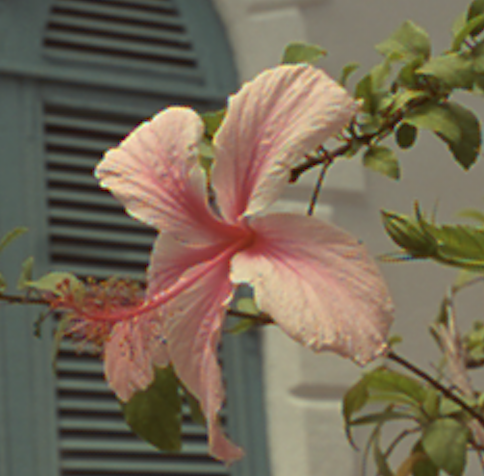
\includegraphics[width=0.5\textwidth]{imagenes/img3_blur.png}
        \caption{}
         \end{center}
\endminipage
\end{figure}


\paragraph{Ringing}

\begin{figure}[h]
\minipage{0.5\textwidth}
\begin{center}
       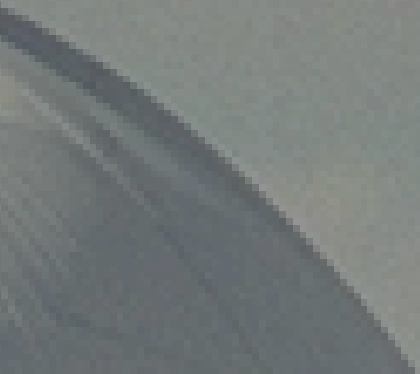
\includegraphics[width=0.5\textwidth]{imagenes/img5_ringing_original.png}
        \caption{Original}
        \end{center}
\endminipage
\minipage{0.5\textwidth}
\begin{center}
       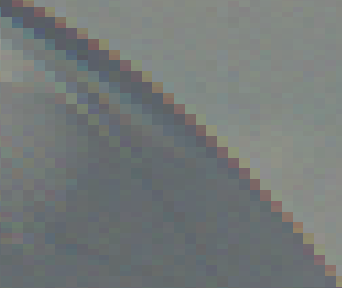
\includegraphics[width=0.5\textwidth]{imagenes/img5_ringing.png}
        \caption{}
         \end{center}
\endminipage
\end{figure}


